%% AMS-LaTeX Created with the Wolfram Language : www.wolfram.com

\documentclass{article}
\usepackage{amsmath, amssymb, graphics, setspace}

\newcommand{\mathsym}[1]{{}}
\newcommand{\unicode}[1]{{}}

\newcounter{mathematicapage}
\begin{document}

\title{Gauss { }Plane { }and { }Complex { }Function}
\author{Graphics { }primitives}
\date{}
\maketitle

\begin{doublespace}
\noindent\(\pmb{b[\text{x$\_\_$}]\text{:=}\text{Map}[\{\text{Re}[\#],\text{Im}[\#]\}\&,x,\{2\}]}\)
\end{doublespace}

\begin{doublespace}
\noindent\(\pmb{\text{bl}[\text{x$\_\_$}]\text{:=}\text{Map}[\text{Line},b[x]]}\)
\end{doublespace}

\begin{doublespace}
\noindent\(\pmb{c[\text{x$\_\_$}]\text{:=}\text{Map}[\{\text{Re}[\#],\text{Im}[\#]\}\&,\text{Transpose}[x],\{2\}]}\)
\end{doublespace}

\begin{doublespace}
\noindent\(\pmb{\text{cl}[\text{x$\_\_$}]\text{:=}\text{Map}[\text{Line},c[x]]}\)
\end{doublespace}

\begin{doublespace}
\noindent\(\pmb{a=\text{Table}[N[i/10]+I N[j/10],\text{(*}I=\text{Sqrt}[-1]\text{*)}\{j,0.1,101,10.1/2\},\{i,0.1,101,10.1/2\}];}\)
\end{doublespace}

\begin{doublespace}
\noindent\(\pmb{\text{plt}[\text{clr$\_$},\text{x$\_\_$}]\text{:=}\text{Show}[\text{Graphics}[\{\text{Hue}[\text{clr}],\text{bl}[x]\}],\text{Graphics}[\{\text{Hue}[\text{clr}],\text{cl}[x]\}],}\\
\pmb{\text{AspectRatio}\text{-$>$}\text{Automatic},\text{Frame}\text{-$>$}\text{True}]}\)
\end{doublespace}

\begin{doublespace}
\noindent\(\pmb{\text{plt}[.75,a]}\)
\end{doublespace}

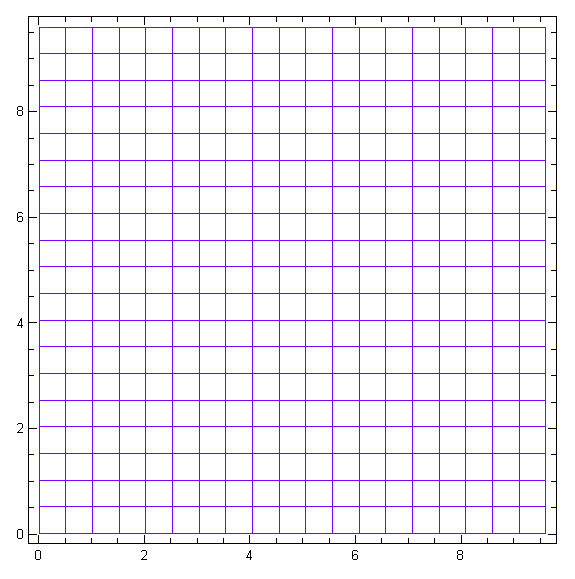
\includegraphics{functions_on_complex-plane_gr1.eps}

\begin{doublespace}
\noindent\(\pmb{r=\text{Exp}[I \text{Pi}*.25]\quad \text{(*}I=\text{Sqrt}[-1]\text{*)}}\)
\end{doublespace}

\begin{doublespace}
\noindent\(0.707107\, +0.707107 i\)
\end{doublespace}

\begin{doublespace}
\noindent\(\pmb{\text{plt}[.75,r*a]}\\
\pmb{\text{(*}\text{Rotate} \text{of} \text{Angle}=\text{Pi}/4 \text{around} \text{zero}.r \text{acts} \text{to} \text{each} \text{element} \text{of}
a\text{*)}}\)
\end{doublespace}

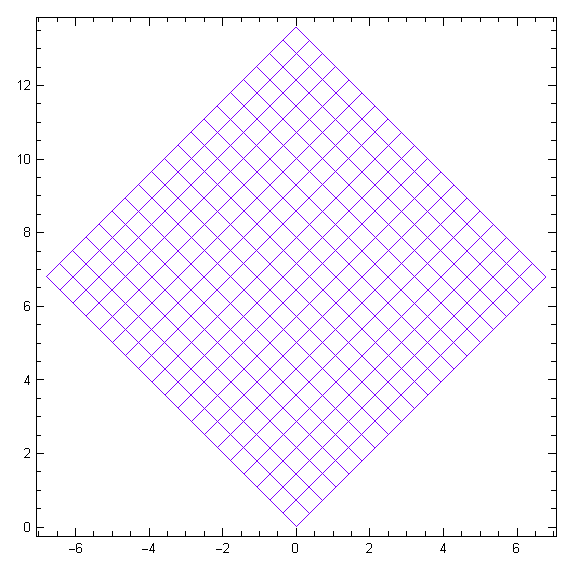
\includegraphics{functions_on_complex-plane_gr2.eps}

\begin{doublespace}
\noindent\(\pmb{\text{plt}[.75,\text{Conjugate}[a]]}\\
\pmb{\text{(*Conjugate acts to each element of a*)}}\)
\end{doublespace}

\includegraphics{functions_on_complex-plane_gr3.eps}

\section*{Function { }acts { }to { }each { }element { }of { }List .}

\begin{doublespace}
\noindent\(\pmb{\text{plt}[.05,\text{Sin}[a]]\quad \text{(*sine function*)}}\)
\end{doublespace}

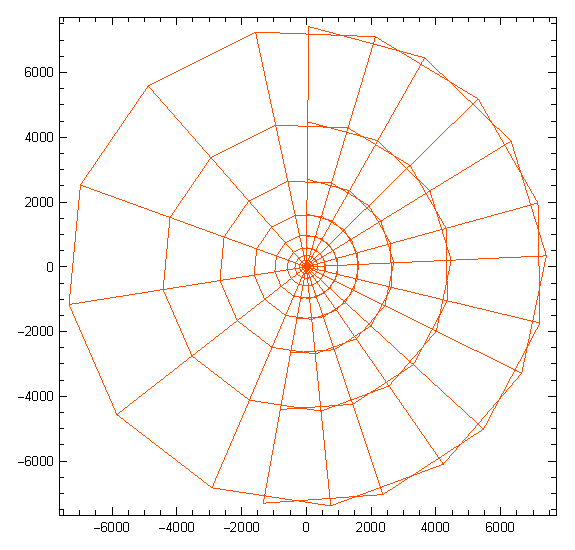
\includegraphics{functions_on_complex-plane_gr4.eps}

\begin{doublespace}
\noindent\(\pmb{\text{g1}=\text{plt}[.9,1/a]\text{  }\text{(*}1/a \text{is} \text{inverse} \text{of} \text{each} \text{element} \text{of} a\text{*)}}\)
\end{doublespace}

\includegraphics{functions_on_complex-plane_gr5.eps}

\begin{doublespace}
\noindent\(\pmb{\text{Show}[\text{g1},\text{PlotRange}\text{-$>$}\{\{0,0.35\},\{-0.35,0\}\}]}\)
\end{doublespace}

\includegraphics{functions_on_complex-plane_gr6.eps}

\begin{doublespace}
\noindent\(\pmb{\text{g2}=\text{plt}[.76,\text{Zeta}[a]]\quad \text{(*}\text{Riemann}'s \text{Zeta} \text{function}\text{*)}}\)
\end{doublespace}

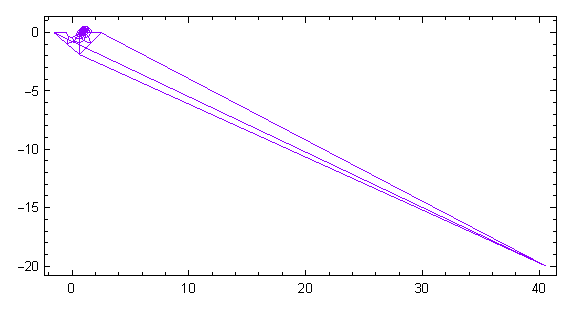
\includegraphics{functions_on_complex-plane_gr7.eps}

\begin{doublespace}
\noindent\(\pmb{\text{Show}[\text{g2},\text{PlotRange}\text{-$>$}\{\{0.5,1.5\},\{-0.2,0.2\}\}]}\)
\end{doublespace}

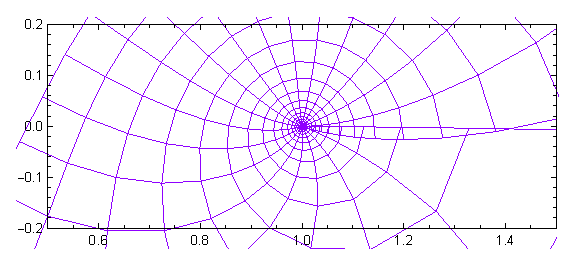
\includegraphics{functions_on_complex-plane_gr8.eps}

\begin{doublespace}
\noindent\(\pmb{?\text{BesselJ}}\)
\end{doublespace}

\begin{doublespace}
\noindent\(\fbox{$$}\)
\end{doublespace}

\begin{doublespace}
\noindent\(\pmb{\text{g3}=\text{plt}[.75,\text{BesselJ}[1,a]]}\)
\end{doublespace}

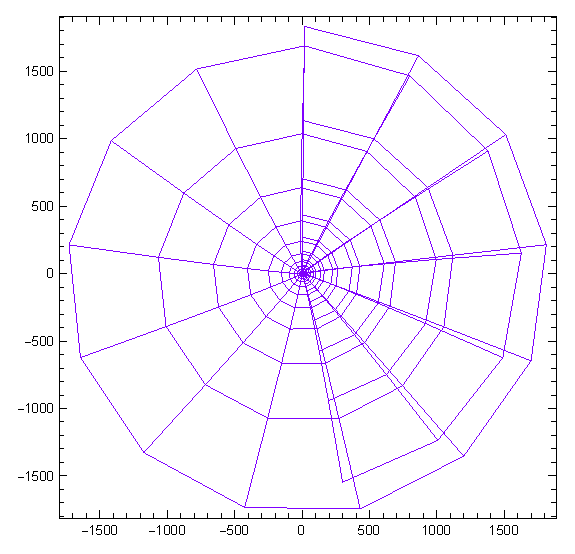
\includegraphics{functions_on_complex-plane_gr9.eps}

\begin{doublespace}
\noindent\(\pmb{\text{Show}[\text{g3},\text{PlotRange}\text{-$>$}\{\{-200,200\},\{-0150,150\}\}]}\)
\end{doublespace}

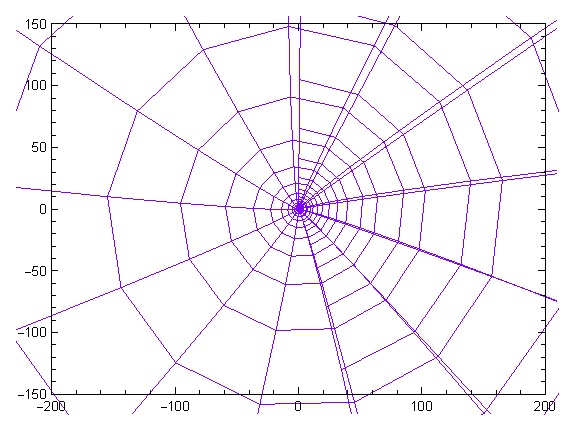
\includegraphics{functions_on_complex-plane_gr10.eps}

\begin{doublespace}
\noindent\(\pmb{\text{plt}[.75,\text{Sqrt}[a]]}\\
\pmb{\text{(*Square Root of each element of a*)}}\)
\end{doublespace}

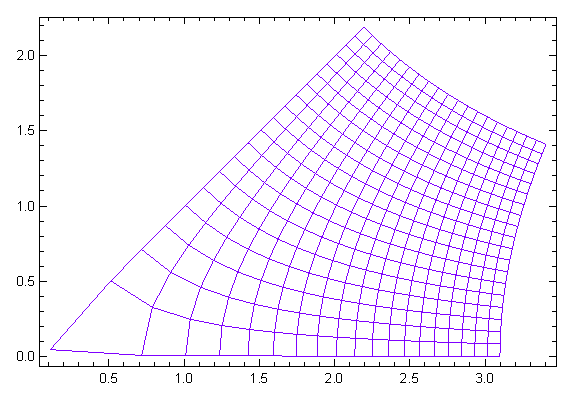
\includegraphics{functions_on_complex-plane_gr11.eps}

\begin{doublespace}
\noindent\(\pmb{\text{plt}[.5,a{}^{\wedge}(.5+I)]\quad \text{(*Power by {``}1/2 + Sqrt[-1]{''}*)}}\)
\end{doublespace}

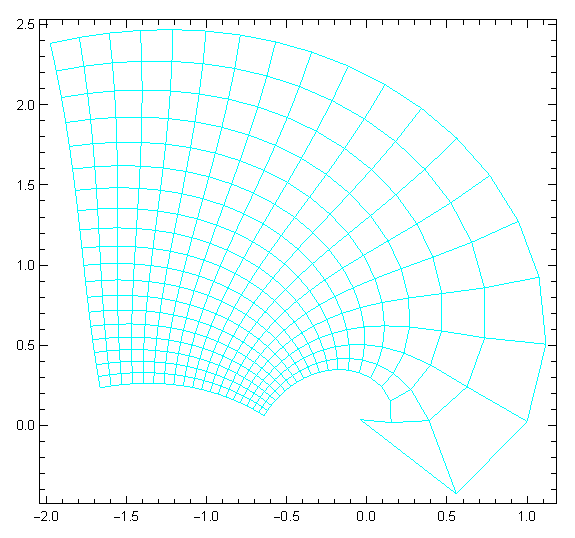
\includegraphics{functions_on_complex-plane_gr12.eps}

\begin{doublespace}
\noindent\(\pmb{?\text{AiryAi}}\)
\end{doublespace}

\begin{doublespace}
\noindent\(\fbox{$$}\)
\end{doublespace}

\begin{doublespace}
\noindent\(\pmb{\text{plt}[.5,\text{AiryAi}[\text{Evaluate}[a/5]]]}\)
\end{doublespace}

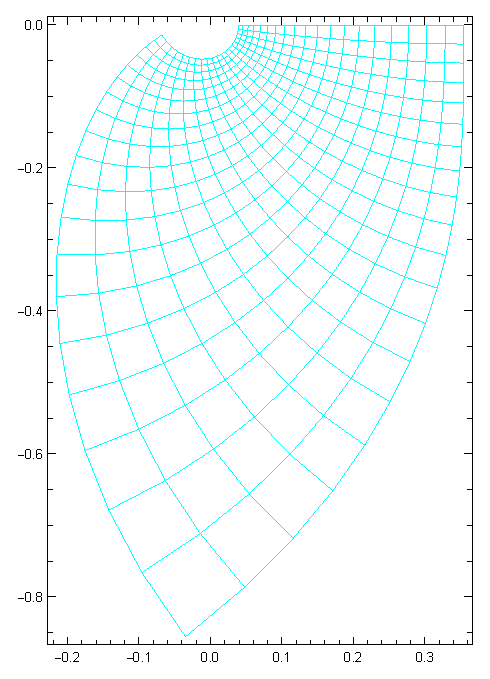
\includegraphics{functions_on_complex-plane_gr13.eps}

\begin{doublespace}
\noindent\(\pmb{\text{a1}=4+4I}\)
\end{doublespace}

\begin{doublespace}
\noindent\(4+4 i\)
\end{doublespace}

\begin{doublespace}
\noindent\(\pmb{\text{a2}=6+7I}\)
\end{doublespace}

\begin{doublespace}
\noindent\(6+7 i\)
\end{doublespace}

\begin{doublespace}
\noindent\(\pmb{\text{g4}=\text{plt}[.25,(a-\text{a1})/(a-\text{a2})]}\)
\end{doublespace}

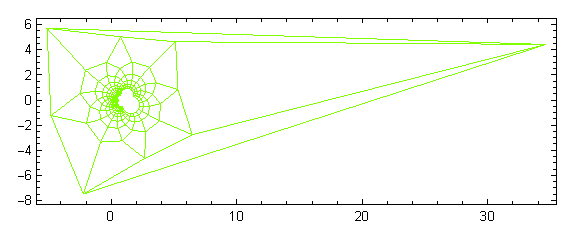
\includegraphics{functions_on_complex-plane_gr14.eps}

\begin{doublespace}
\noindent\(\pmb{\text{Show}[\text{g4},\text{PlotRange}\text{-$>$}\{\{-1.5,3\},\{-3,3\}\}]}\)
\end{doublespace}

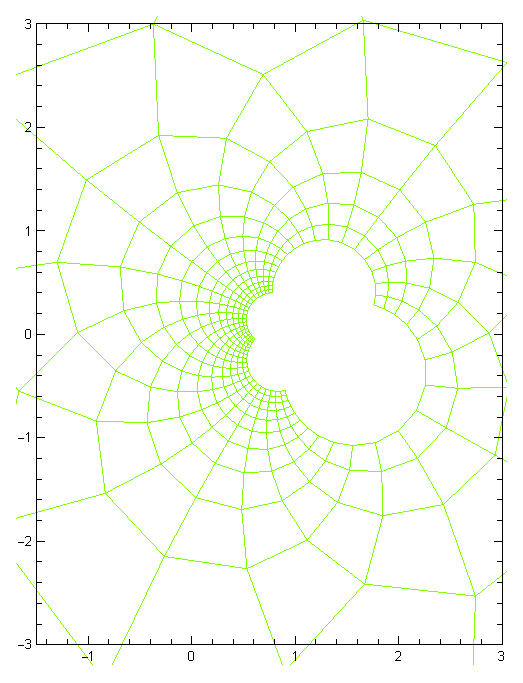
\includegraphics{functions_on_complex-plane_gr15.eps}

\end{document}
